\documentclass[11pt,a4paper]{article}
\usepackage[utf8]{inputenc}
\usepackage[T1]{fontenc}
\usepackage{amsmath,amssymb}
\usepackage{graphicx}
\usepackage{xcolor}
\usepackage{color}
\usepackage{hyperref}
\usepackage{geometry}
\usepackage{tikz}
\usepackage{enumitem}
\usepackage{float}
\usepackage{listings}
\usepackage{caption}
\usepackage{booktabs}
\usepackage{longtable}
\usepackage{fancyhdr}
\geometry{margin=2.0cm,columnsep=0.7cm}
\usetikzlibrary{shapes,arrows,positioning,fit,backgrounds,calc,shadows,decorations.pathreplacing}
\hypersetup{colorlinks=true,linkcolor=blue,urlcolor=blue,citecolor=blue}
\definecolor{legacycolor}{RGB}{220,80,80}
\definecolor{refactorcolor}{RGB}{60,140,80}
\definecolor{sharedcolor}{RGB}{80,120,180}
\definecolor{configcolor}{RGB}{200,140,40}
\definecolor{simcolor}{RGB}{140,80,180}
\definecolor{codebg}{RGB}{245,245,245}
\lstset{basicstyle=\ttfamily\small,backgroundcolor=\color{codebg},frame=single,breaklines=true}
\title{\textbf{Weekly Report}\\[4pt]\large QCar Refactor \& CARLA Simulation}
\author{Qi LI}
\date{\today}
\begin{document}
\twocolumn[
\maketitle
\tableofcontents
\vspace{1em}
]
\small
\section{Work summary}
\begin{itemize}
    \item Vehicle lifecycle queries were separated from IO, estimation, planning, control, and V2V modules. Meanwhile, the platform is software-free and easy to extend.
    \item Carla support was added, and a v2v test is implemented.
\end{itemize}
\section{Platform refactor}

\subsection{Platform redesign}
The old platform put most vehicle work inside one large \texttt{VehicleLogic} class. This made small changes risky and made it hard to test a module on its own.

% Standard self-contained color definitions for legacy diagram
\definecolor{legacyred}{RGB}{192, 57, 43}
\definecolor{legacybg}{RGB}{253, 237, 236}
\definecolor{darkgray}{RGB}{44, 62, 80}
\definecolor{bordergray}{RGB}{189, 195, 199}

\begin{figure}[H]
\centering
\resizebox{\columnwidth}{!}{%
\begin{tikzpicture}[
    font=\sffamily\footnotesize,
    node distance=0.8cm,
    auto,
    % Clean styled submodules
    box/.style={
        rectangle, 
        draw=legacyred!60, 
        fill=legacybg, 
        text=legacyred!85!black, 
        text width=2.8cm, 
        align=center, 
        minimum height=0.85cm, 
        rounded corners=3pt,
        line width=0.8pt
    },
    % Bold central monolithic hub
    bigbox/.style={
        rectangle, 
        draw=legacyred, 
        fill=legacyred!10, 
        text=legacyred!85!black, 
        text width=3.8cm, 
        align=center, 
        minimum height=1.4cm, 
        font=\bfseries, 
        rounded corners=5pt, 
        line width=1.3pt
    },
    arrow/.style={
        ->, 
        >=stealth, 
        thick, 
        draw=legacyred!80
    }
]
    % Central Hub
    \node[bigbox] (vl) at (0,0) {\textbf{MONOLITHIC HUB}\\\texttt{VehicleLogic}\\};

    % Left Column (Symmetrical outer offsets)
    \node[box] (io) at (-4.5, 1.8) {Hardware IO\\\texttt{self.qcar}};
    \node[box] (obs) at (-4.5, 0.6) {Observer\\EKF / KalmaNet};
    \node[box] (v2v) at (-4.5, -0.6) {V2V Manager\\+ Attack Module};
    \node[box] (gs) at (-4.5, -1.8) {Ground Station\\TCP Client};

    % Right Column (Symmetrical outer offsets)
    \node[box] (ctrl) at (4.5, 1.8) {Controller\\PID / Stanley};
    \node[box] (sm) at (4.5, 0.6) {StateMachine\\12 state files};
    \node[box] (yolo) at (4.5, -0.6) {YOLO\\Perception};
    \node[box] (other) at (4.5, -1.8) {Platoon / Taxi\\Calibration / SysID};
    
    % Outward radiating arrows from center (zero overlapping lines)
    \draw[arrow] (vl.west) -- (io.east);
    \draw[arrow] (vl.west) -- (obs.east);
    \draw[arrow] (vl.west) -- (v2v.east);
    \draw[arrow] (vl.west) -- (gs.east);
    
    \draw[arrow] (vl.east) -- (ctrl.west);
    \draw[arrow] (vl.east) -- (sm.west);
    \draw[arrow] (vl.east) -- (yolo.west);
    \draw[arrow] (vl.east) -- (other.west);
\end{tikzpicture}
}
\caption{Before: one \texttt{VehicleLogic} class directly handled every subsystem.}
\label{fig:legacy}
\end{figure}

\begin{enumerate}[leftmargin=*]
    \item \textbf{One large main class.} \texttt{VehicleLogic} handled the lifecycle, sensors, observer, state machine, controller, V2V, telemetry, logging, and optional research features.
    {\color{blue} The main loop grew to more than 800 lines, so it was difficult to review.}

    \item \textbf{Modules were tightly connected.} A change in one feature could break an unrelated feature.

    \item \textbf{Data flow was mixed.} Changing sensor data or V2V data required edits in several modules.

    \item \textbf{Configuration was scattered.} Selecting a backend or controller meant searching several files.

    \item \textbf{Simulation and hardware were mixed.} Adding a simulator could require changing the core runtime.
\end{enumerate}

The figure shows why the old structure was difficult to extend: the main class talks directly to every subsystem.


\subsection{What I built}

I moved the main lifecycle into a small \texttt{VehicleRuntime}. It starts, steps, and stops the vehicle. The state machine only decides whether driving is safe. IO, observer, planner, controller, and V2V are now separate modules built by the module factory.

% Standard self-contained color definitions for refactored diagram
\definecolor{configcolor}{RGB}{230, 126, 34}    % Warm amber
\definecolor{refactorcolor}{RGB}{39, 174, 96}   % Fresh green
\definecolor{sharedcolor}{RGB}{41, 128, 185}     % Academic blue
\definecolor{simcolor}{RGB}{142, 68, 173}        % Plum/purple
\definecolor{darkgray}{RGB}{44, 62, 80}
\definecolor{lightgray}{RGB}{245, 247, 250}
\definecolor{bordergray}{RGB}{189, 195, 199}

\begin{figure}[H]
\centering
\resizebox{\columnwidth}{!}{%
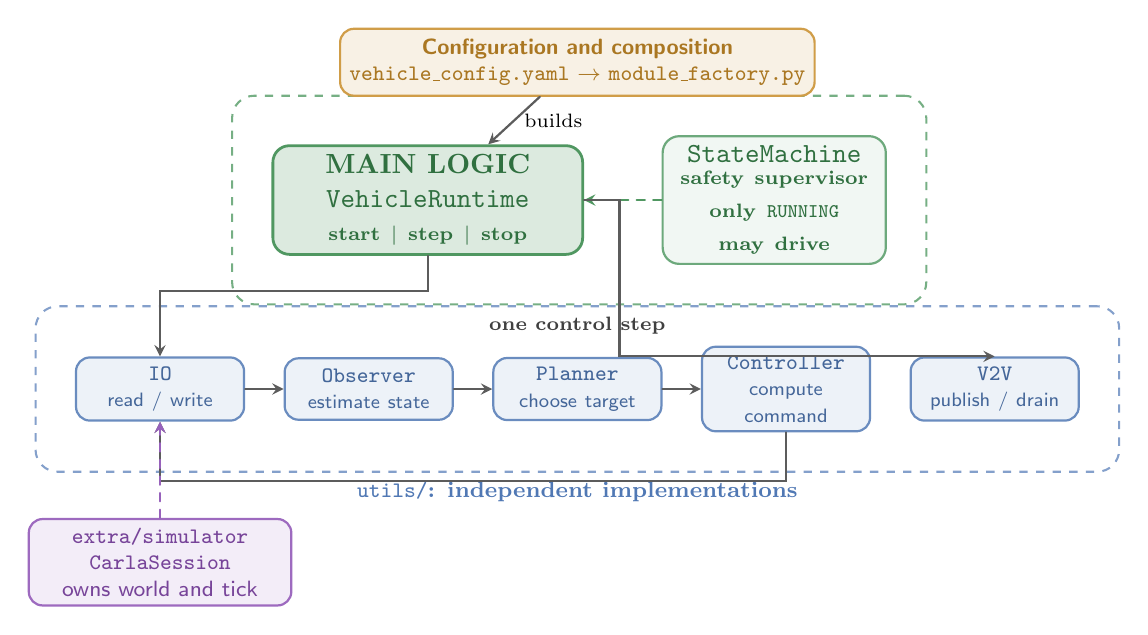
\begin{tikzpicture}[
    font=\sffamily\footnotesize,
    config/.style={rectangle, draw=configcolor!85, fill=configcolor!12, text=configcolor!85!black, rounded corners=5pt, minimum width=5.1cm, minimum height=0.85cm, align=center, line width=.8pt},
    mainlogic/.style={rectangle, draw=refactorcolor!90, fill=refactorcolor!18, text=refactorcolor!80!black, rounded corners=6pt, text width=3.7cm, minimum height=1.0cm, align=center, font=\bfseries, line width=1pt},
    safety/.style={rectangle, draw=refactorcolor!75, fill=refactorcolor!7, text=refactorcolor!80!black, rounded corners=6pt, text width=2.6cm, minimum height=1.0cm, align=center, font=\bfseries, line width=.8pt},
    utility/.style={rectangle, draw=sharedcolor!85, fill=sharedcolor!10, text=sharedcolor!85!black, rounded corners=5pt, text width=1.9cm, minimum height=.78cm, align=center, line width=.8pt},
    external/.style={rectangle, draw=simcolor!85, fill=simcolor!10, text=simcolor!85!black, rounded corners=5pt, text width=3.1cm, minimum height=.8cm, align=center, line width=.8pt},
    frame/.style={draw=#1!70, dashed, rounded corners=8pt, line width=.75pt, inner sep=5mm},
    flow/.style={->, >=stealth, draw=darkgray!85, line width=.8pt, line cap=round},
    safetyflow/.style={->, >=stealth, draw=refactorcolor!90, dashed, line width=.8pt, line cap=round},
    externalflow/.style={->, >=stealth, draw=simcolor!90, dashed, line width=.8pt, line cap=round}
]
    \node[config] (compose) at (0,3.1) {\textbf{Configuration and composition}\\\texttt{vehicle\_config.yaml} $\rightarrow$ \texttt{module\_factory.py}};

    \node[mainlogic] (runtime) at (-1.9,1.35) {\textbf{MAIN LOGIC}\\\texttt{VehicleRuntime}\\\scriptsize start $\vert$ step $\vert$ stop};
    \node[safety] (sm) at (2.5,1.35) {\texttt{StateMachine}\\\scriptsize safety supervisor\\\scriptsize only \texttt{RUNNING} may drive};

    \node[font=\scriptsize\bfseries,text=darkgray] at (0,-.25) {one control step};
    \node[utility] (io) at (-5.3,-1.05) {\texttt{IO}\\\scriptsize read / write};
    \node[utility] (observer) at (-2.65,-1.05) {\texttt{Observer}\\\scriptsize estimate state};
    \node[utility] (planner) at (0,-1.05) {\texttt{Planner}\\\scriptsize choose target};
    \node[utility] (controller) at (2.65,-1.05) {\texttt{Controller}\\\scriptsize compute command};
    \node[utility] (v2v) at (5.3,-1.05) {\texttt{V2V}\\\scriptsize publish / drain};

    \node[external] (session) at (-5.3,-3.25) {\texttt{extra/simulator}\\\texttt{CarlaSession} owns world and tick};

    \begin{scope}[on background layer]
        \node[frame=refactorcolor, fit=(runtime)(sm), label={[font=\footnotesize\bfseries,text=refactorcolor]above:\texttt{core/}: orchestration and safety}] {};
        \node[frame=sharedcolor, fit=(io)(observer)(planner)(controller)(v2v), label={[font=\footnotesize\bfseries,text=sharedcolor]below:\texttt{utils/}: independent implementations}] {};
    \end{scope}

    \draw[flow] (compose) -- node[right, font=\scriptsize] {builds} (runtime);
    \draw[safetyflow] (sm.west) -- (runtime.east);
    \draw[flow] (runtime.south) -- ++(0,-.45) -| (io.north);
    \draw[flow] (io) -- (observer);
    \draw[flow] (observer) -- (planner);
    \draw[flow] (planner) -- (controller);
    \draw[flow] (controller.south) -- ++(0,-.62) -| (io.south);
    \draw[flow] (runtime.east) -- ++(.45,0) |- (v2v.north);
    \draw[externalflow] (session) -- (io);

\end{tikzpicture}
}
\caption{After: \texttt{core/} keeps the main logic; \texttt{utils/} holds replaceable modules.}
\label{fig:refactor}
\end{figure}

\subsection{Multi-vehicle simulation}

Before, the scenario configuration need to be made manually by running the command with parsers. I added scenarios configuration and \texttt{VehicleProcessSpec} so each vehicle runs in its own process with its own \texttt{VehicleRuntime}. This keeps each control loop independent while allowing V2V communication. In CARLA, one process owns the world tick.

% Standard color definitions for multi-vehicle support
\definecolor{primary}{RGB}{41, 128, 185}
\definecolor{secondary}{RGB}{39, 174, 96}
\definecolor{accent}{RGB}{211, 84, 0}
\definecolor{darkgray}{RGB}{44, 62, 80}
\definecolor{lightgray}{RGB}{245, 247, 250}
\definecolor{bordergray}{RGB}{189, 195, 199}

\begin{figure}[H]
\centering
\resizebox{\columnwidth}{!}{%
\begin{tikzpicture}[
    font=\sffamily\footnotesize,
    node distance=0.8cm,
    box/.style={
        rectangle, 
        draw=bordergray, 
        fill=lightgray, 
        text=primary!85!black, 
        text width=4.2cm, 
        align=center, 
        minimum height=0.8cm, 
        rounded corners=3pt,
        line width=0.8pt
    },
    corebox/.style={
        rectangle, 
        draw=secondary, 
        fill=secondary!10, 
        text=secondary!80!black, 
        text width=3.2cm, 
        align=center, 
        minimum height=0.8cm, 
        font=\bfseries, 
        rounded corners=3pt,
        line width=1.1pt
    },
    arrow/.style={
        ->, 
        >=stealth, 
        thick, 
        draw=darkgray!80
    },
    v2v_arrow/.style={
        <->, 
        >=stealth, 
        dashed, 
        thick, 
        draw=primary
    }
]
    \node[box] (scenario) at (0,0) {\textbf{\texttt{scenario.yaml}}\\vehicles, spawns, routes,\\V2V endpoints, tick owner};

    \node[box, below=1.2cm of scenario, xshift=-3.5cm] (virtual) {\textbf{\texttt{VirtualRunner}}\\Local processes};
    \node[box, below=1.2cm of scenario, xshift=3.5cm] (carla) {\textbf{\texttt{CarlaRunner}}\\shared CARLA world\\one process owns the tick};

    \node[box, below=0.8cm of virtual] (spec1) {\texttt{VehicleProcessSpec}\\vehicle\_id=0, ...};
    \node[box, below=0.8cm of carla] (spec2) {\texttt{VehicleProcessSpec}\\vehicle\_id=1, ...};

    \node[corebox, below=0.8cm of spec1] (rt1) {\texttt{VehicleRuntime}\\\scriptsize Process 1: independent control loop};
    \node[corebox, below=0.8cm of spec2] (rt2) {\texttt{VehicleRuntime}\\\scriptsize Process 2: independent control loop};
    \node[draw=secondary!65, dashed, rounded corners=6pt, inner sep=4mm, fit=(spec1)(rt1),
          label={[font=\scriptsize\bfseries,text=secondary]below:Vehicle process 1}] {};
    \node[draw=secondary!65, dashed, rounded corners=6pt, inner sep=4mm, fit=(spec2)(rt2),
          label={[font=\scriptsize\bfseries,text=secondary]below:Vehicle process 2}] {};

    \draw[v2v_arrow, bend left=18] (rt1.30) to node[above, font=\scriptsize\bfseries\ttfamily, text=primary] {UDP V2V} (rt2.150);

    \draw[arrow] (scenario.south) -- ++(0,-0.4) -| (virtual.north);
    \draw[arrow] (scenario.south) -- ++(0,-0.4) -| (carla.north);
    
    \draw[arrow] (virtual) -- (spec1);
    \draw[arrow] (carla) -- (spec2);
    \draw[arrow] (spec1) -- (rt1);
    \draw[arrow] (spec2) -- (rt2);

\end{tikzpicture}
}
\caption{One scenario starts separate vehicle processes. V2V connects them.}
\label{fig:multi}
\end{figure}

\subsection{What is complete}

This is the current status of the refactor work.

\begin{table}[H]
\centering\scriptsize
\setlength{\tabcolsep}{2pt}
\begin{tabular}{@{}p{2.0cm}p{1.1cm}p{4.5cm}@{}}
\toprule
\textbf{Step} & \textbf{State} & \textbf{Key outcome} \\
\midrule
Configuration & Done & YAML profiles and validation \\
Contracts & Done & Shared dataclasses \\
Runtime & Done & Runtime coordinator and module factory \\
IO adapters & Done & QCar, virtual, and CARLA backends \\
CARLA & Done & Session, adapter, smoke/control tests \\
Multi-vehicle & Done & Process specs and YAML scenarios \\
V2V / fleet & Partial & UDP transport; fleet work pending \\
Ground station & Planned & Bridge and visual application pending \\
\bottomrule
\end{tabular}
\caption{Current implementation status.}
\label{tab:status}
\end{table}

\subsection{Still to do}

\begin{itemize}[leftmargin=*]
    \item \textbf{Fleet features}: peer membership, fleet snapshots, stale-peer removal, and payload decoding.
    \item \textbf{Ground-station bridge}: Vehicle-side TCP bridge with MessagePack framing, command queue, telemetry queue.
    \item \textbf{Ground-station application}: Visual telemetry display and command interface.
    \item \textbf{Physical QCar2}: the licence is expired, so I kept this code as reference only.
    \item \textbf{ROS adapters}: Deferred until external ROS transport contracts are defined.
    \item \textbf{Operation strategies}: Platoon, manual mode, taxi, and calibration as pluggable strategies behind the RUNNING state.
\end{itemize}

\section{CARLA integration}

I checked CARLA in stages. Unit tests use fake CARLA objects, so they run without a server. Then direct-run tests use a local CARLA server and save CSV files and plots for review.

\begin{figure}[H]
\centering
\resizebox{\columnwidth}{!}{%
\begin{tikzpicture}[
    font=\sffamily\footnotesize,
    test/.style={rectangle, draw=primary!85, fill=primary!8, text=primary!85!black, rounded corners=5pt, text width=3.25cm, minimum height=.9cm, align=center, line width=.8pt},
    live/.style={rectangle, draw=accent!85, fill=accent!8, text=accent!85!black, rounded corners=5pt, text width=3.25cm, minimum height=.95cm, align=center, line width=.8pt},
    artifact/.style={rectangle, draw=secondary!85, fill=secondary!9, text=secondary!80!black, rounded corners=5pt, text width=4.1cm, minimum height=.82cm, align=center, line width=.8pt},
    frame/.style={draw=#1!70, dashed, rounded corners=8pt, line width=.75pt, inner sep=4mm},
    arrow/.style={->, >=stealth, draw=darkgray!85, line width=.8pt, line cap=round}
]
    % Unit tests: all dependencies replaced by fakes.
    \node[test] (sessionunit) at (-2.0,2.1) {\textbf{Session lifecycle}\\\scriptsize fake client, world, and actors};
    \node[test] (iounit) at (2.0,2.1) {\textbf{CARLA IO adapter}\\\scriptsize fake actor and sensor snapshot};
    \node[font=\small\bfseries,text=primary] at (0,3.20) {1. Unit tests --- no CARLA server required};

    % Live single-vehicle tests.
    \node[live] (smoke) at (-4.25,.05) {\textbf{Smoke and IO trace}\\\scriptsize spawn, tick, read, safe cleanup};
    \node[live] (control) at (0,.05) {\textbf{Closed-loop control}\\\scriptsize EKF + planner + controller};
    \node[live] (entry) at (4.25,.05) {\textbf{Production entry point}\\\scriptsize config $\rightarrow$ factory $\rightarrow$ runtime};
    \node[font=\small\bfseries,text=accent] at (0,1.10) {2. Live single-vehicle CARLA tests};

    % Multi-process tests.
    \node[live] (multi) at (-2.0,-2.05) {\textbf{Two vehicle processes}\\\scriptsize one tick owner, distinct trajectories};
    \node[live] (v2vtest) at (2.0,-2.05) {\textbf{V2V diagnostics}\\\scriptsize latency, sequence gaps, packet loss};
    \node[font=\small\bfseries,text=accent] at (0,-1.08) {3. Live multi-process scenario tests};

    \node[artifact] (artifacts) at (0,-3.65) {\textbf{Reviewable evidence}\\CSV sensor/control traces, trajectory plots, V2V latency and packet-loss diagnostics};

    \draw[arrow] (0,1.55) -- (0,.68);
    \draw[arrow] (0,-.62) -- (0,-1.42);
    \draw[arrow] (0,-2.60) -- (artifacts.north);
\end{tikzpicture}
}
\caption{CARLA checks: fakes first, then live single-vehicle and multi-vehicle runs.}
\label{fig:carla-tests}
\end{figure}

The first saved plot shows the closed-loop control run. It compares the planned path, GPS, EKF, speed, commands, and position error.

\begin{figure}[H]
\centering

\includegraphics[width=\columnwidth]{../test/artifacts/integration_carla_control.png}
\caption{Closed-loop CARLA control result.}
\label{fig:carla-control-artifact}
\end{figure}

The multi-vehicle run also records the V2V path, latency, queue delay, and packet loss.

\begin{figure}[H]
\centering

\includegraphics[width=\columnwidth]{../test/artifacts/carla_multi_process_v2v/peer_state_latency_loss.png}
\caption{Two-vehicle CARLA V2V result.}
\label{fig:carla-v2v-artifact}
\end{figure}

The unit and integration tests are under \texttt{test/}. This gives me a quick way to find whether a problem comes from the algorithm, runtime, or simulator before running a larger scenario.


\section{Conclusion}
\subsection{Next steps}
\begin{itemize}
    \item Finish fleet building and the ground-station path in the refactored structure.
    
    {\color{blue} Will be finished in this week.}

    \item Test the refactored code on QCar2 hardware when the licence is available.
    
    {\color{blue} Will be finished in two weeks.}

    \item Study 2D platoon control and build a distributed high-gain observer.
    
    {\color{blue} Will be finished in two weeks.}

    \item Use MATLAB to test the observer before moving it into the vehicle platform.
    
    {\color{blue} Will be finished in two weeks.}
\end{itemize}
The refactored platform is now running with CARLA. Next, I will finish the fleet and ground-station features and test the platform on QCar2 hardware.

I will first test the longitudinal fleet system. Then I will formulate the triangular form for the 2D fleet system and validate it in MATLAB. After that, I will test it in CARLA simulation, and finally on QCar2 hardware.

I am currently reading E.D. Sontag’s tutorial on stability. After that, I will investigate whether an interval observer with more advanced design methods can provide better stability. This could be practical for the vehicle platform and also help me enter the observer-design research field.

\end{document}
